%%%%%%%%%%%%%%%%%%%%%%%%%%%%%%%%%%%%%%%%%%%%%%%%%%%%%%%%%%%%%%%%%%%%%%%%%%%%%%%%%
%
% This is a very basic template for mathematical presentations using LaTeX and beamer, aimed at University of Edinburgh students on the Honours Analysis course 2017-2018, for their "Skills" presentations.
%
% This template is just to get you started and to see what the possibilities are.  There is no required format, and you are free to use, discard, edit as much as you like.  I've put in some mathematical content to demonstrate the very basics of LaTeX.  Clearly, you will need to change this.
%
% Except for a few structural comments, I don't comment on the LaTeX itself.  If you have used it before, most of what you know should apply as usual.  If you have not, have a look at the source code, the output, and experiment with editing the code and see what happens.  Most LaTeX code is pretty intuitive, e.g. the command to produce an alpha is \alpha, the command for an integral sign is \int, etc.  You can learn an awful lot by guesswork, trial and error, and google.  
%
% The percent signs "%" are comment signs, and instruct LaTeX to ignore everything following the sign on the same line.  They can be used to comment on the code.
%
%%%%%%%%%%%%%%%%%%%%%%%%%%%%%%%%%%%%%%%%%%%%%%%%%%%%%%%%%%%%%%%%%%%%%%%%%%%%%%%%
%
% The following lines are the preamble.  They help LaTeX set-up the document, but do not print anything yet.
\usepackage[spanish]{babel}
\usepackage[utf8x]{inputenc}
\documentclass{beamer}		% This tells LaTeX the document will be a "beamer" presentation

\usetheme{Madrid}		% Sets basic formatting.  Lots of options, google "beamer themes"

\usecolortheme{dolphin}	% Sets the colour scheme.  Lots of options, google "beamer color themes"

\setbeamertemplate{navigation symbols}{}	% Manually changes one piece of formatting.  See what the difference is by commenting this line out.

\date{21 de febrero de 2019}	% Insert the date of your presentation. \today gives an unsurprising automatic date.

\title[Parametrizaci\'on]{M\'etodo de parametrizaci\'on:\\Variedades estables e inestables en mapeos Hamiltonianos de dos dimensiones}	% Insert your title.  Depending on the theme you choose above, a "short title" might be useful, as it will appear on the footer of each slide.

\author[E. \'Alvarez]{Evelyn \'Alvarez Cruz} % Insert your name

\institute[FC]{Facultad de Ciencias\\ Universidad Nacional Aut\'onoma de M\'exico} % Self-explanatory
\usepackage[spanish]{babel}
\newtheorem{teorema}[theorem]{Teorema}
\usepackage[utf8x]{inputenc}
\begin{document} 	% Let's begin

% Presentations come in slide frames.  You have to tell LaTeX when to start a frame, and when to end the frame.  The most common error beginners make with beamer is forgetting the \end{frame} command.	

\begin{frame}	

\titlepage	% Prints a title page populated with the information given in the preamble
	
\end{frame}	

%--------------------------------------------------------------------------
\begin{frame}{Resumen}	
\begin{itemize}
    \item[1] Motivaciones.
    \item[2] El m\'etodo de parametrizaci\'on.
    \begin{itemize}
        \item[2.1] Ejemplo de aplicaci\'on al mapeo est\'andar. 
    \end{itemize}
    \item[3] Implementaci\'on
    \item[4] Ejemplos
    \begin{itemize}
        \item[4.1] El mapeo est\'andar
        \item[4.2] El mapeo de H\'enon
        \item[4.3] El mapeo exponencial
    \end{itemize}
    \item[5] Conclusiones y perspectivas
\end{itemize}

\end{frame}



%-----------------------------------------------------------------------





%----------------------------------------------------------------------------------------------------------
\begin{frame}{Motivaciones}	
\begin{itemize}
    \item Los mapeos discretos pueden describir sistemas f\'isicos.\\
    \begin{figure}
        \centering
        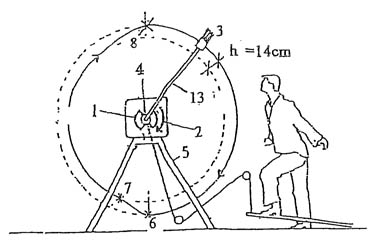
\includegraphics[scale=1.5]{kicked.jpg}
        \includegraphics[scale=.1]{fluid.png}
        \label{fig:rotor}
    \end{figure}
    \item Conocer la din\'amica alrededor de puntos fijos.\\
    
    \item Conocer el comportamiento de las variedades estables e inestables asociadas a puntos fijos hiperb\'olicos.\\
    
    \item Los m\'etodos mediante los cuales se calculan las variedades son iterativos.\\
\end{itemize}

\end{frame}
%------------------------------------------------------------------------------------------
\begin{frame}{M\'etodo de parametrizaci\'on}
Sea $\mathbf{f}:\mathbb{R}^{2}\rightarrow\mathbb{R}^{2}$ un mapeo Hamiltoniano, el cual tiene un punto fijo hiperb\'olico $\mathbf{x}_{*}$.\\
\begin{teorema}{Hartman-Grobman}
Sea $\mathbf{x}_{*}$ un punto fijo hiperb\'olico de $\mathbf{f}$ y suponga que $\mathbf{f'}(\mathbf{x_{*}})=\lambda$ con $ \vert \lambda_{1}\vert\neq 0,1 $. Entonces hay vecindades $U$ de $\mathbf{x_{*}}$ y $V$ de $0\in\mathbb{R}$ y un homeomorfismo $h:U\rightarrow\mathbb{R}$ que conjuga $\mathbf{f}$ en $U$ con el mapeo lineal $L(\mathbf{x})=\lambda\mathbf{x}$  en $V$.
\end{teorema}
Tomando en cuenta lo anterior
\begin{equation}
    \mathbf{x}_{n+1} =\mathbf{A}\mathbf{x}_{n}, \quad \mathbf{A}=D\mathbf{f}(\mathbf{x}_{*})
    \label{sistema_lineal}
\end{equation}
y sean \\
\begin{equation}
    \vert \lambda_{1}\vert<1 \quad \rightarrow \mathbf{u}
\label{primer_valorp}
\end{equation}
\begin{equation}
    \vert \lambda_{2}\vert<1 \quad \rightarrow \mathbf{v}
\label{primer_valorp}
\end{equation}

\end{frame}
\begin{frame}{M\'etodo de parametrizaci\'o}
    

\begin{figure}
    \centering
    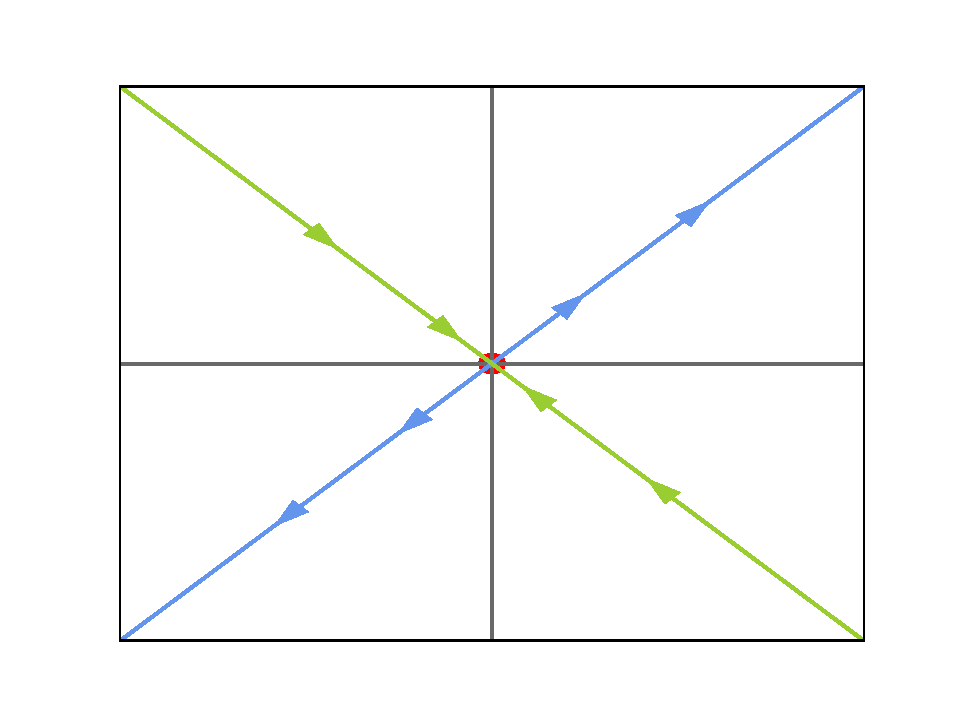
\includegraphics[scale=0.35]{hyperbolic2.pdf}
    \caption{Punto fijo hiperb\'olico.}
    \label{hiperbolico}
\end{figure}
Al rededor de este punto fijo existen dos conjuntos invariantes, la variedad \textbf{estable} y la \textbf{inestable}.\\

\begin{definition}

\end{definition}

\end{frame}  
\begin{frame}{Frame}
\begin{definition}	% There are lots of "theorem-like" environments for beamer just as 	usual with LaTeX: definition, theorem, lemma, example, proof, etc...

A sequence of functions $f_n \colon \mathbb{R} \to \mathbb{R}$ \emph{converges uniformly} to a function $f \colon \mathbb{R} \to \mathbb{R}$ if for all $\epsilon > 0$ there exists an $N \in \mathbb{N}$ such that $n \geq N$ implies 
\[
\sup_{x \in \mathbb{R}} |f_n(x) - f(x)| < \epsilon.
\]

\end{definition}

\pause	% Generates a break in the slide presentation

\begin{block}{Pointwise and uniform continuity} % Blocks are a beamer speciality.

\begin{itemize}
\item Uniform convergence implies pointwise convergence
\item Pointwise convergence does not imply uniform convergence
\end{itemize}

\end{block}

\pause

\begin{theorem}
Let $f_n \colon\mathbb{R} \to \mathbb{R}$ be continuous and converge uniformly to $f \colon \mathbb{R} \to \mathbb{R}$.  Then $f$ is continuous.
\end{theorem}

\end{frame}

\begin{frame}{Uniform convergence and continuity}

\begin{proof}
Let $x \in \mathbb{R}$ and let $\epsilon > 0$.  There exists $N \in \mathbb{N}$ such that $n \geq N$ implies
\begin{equation}
\label{eq1}
\sup_{x \in \mathbb{R}} |f_n(x) - f(x)| < \frac{\epsilon}{3}.
\end{equation}

There exists $\delta > 0$ such that 
\begin{equation}
\label{eq2}
|f_N(x) - f_N(y) | < \frac{\epsilon}{3}\ \mbox{whenever}\ |x-y| < \delta.
\end{equation}

Then inequalities \eqref{eq1} and \eqref{eq2} imply that whenever $|x-y | < \delta$, we have 
\begin{align*}
|f(x) - f(y)| 
& \leq |f(x) - f_N(x)| + |f_N(x) - f_N(y)| + | f_N(y) - f(y) | \\
& < \frac{\epsilon}{3} + \frac{\epsilon}{3} + \frac{\epsilon}{3} \\
& = \epsilon.
\end{align*} 
\end{proof}

\end{frame}

\begin{frame}{People}

This subject owes much to 

\begin{columns}	% A handy way of putting things side-by-side

\begin{column}{0.4\textwidth} % this says the column will be the width of 0.4 times the \textwidth
\begin{figure}	% for graphics
\includegraphics[height=4cm]{Cauchy}	% save your image file in your project, and include using \includegraphics{filename}.  Specify height, width, scaling as shown.
\caption{Augustin-Louis Cauchy}	% there are ways to delete the "Figure:" if you want to
\end{figure}
\end{column}

\begin{column}{0.4\textwidth}
\begin{figure}
\includegraphics[height=4cm]{Weierstrass}
\caption{Karl Weierstrass}
\end{figure}
\end{column}

\end{columns}

\end{frame}
\end{document}	% Done!